% !TeX spellcheck = en_GB
\ifcsname SlidesDistr\endcsname%
	\documentclass[handout,aspectratio=169]{beamer}
\else%
	\documentclass[aspectratio=169]{beamer}
\fi%
\usepackage{fontspec}
\usepackage[T1]{fontenc}
\usepackage{amsmath}
\usepackage{amsfonts}
\usepackage{amssymb}
\usepackage{graphicx}
\usepackage{csquotes}
\usepackage{booktabs}
\usepackage{multicol}
\usepackage{enumerate}
\usepackage{microtype}
\usepackage[labelfont=bf,font={small}]{caption}
\usepackage{hyperref}
\usepackage{booktabs}
\usepackage{subcaption}
\usepackage{fancyhdr}
\usepackage{pdfpages}
\usepackage{siunitx}
\usepackage{tikz}
\usepackage{mdframed}

\defaultfontfeatures{Mapping=tex-text}
\newfontfamily\symbolfont{Symbola}
\newfontfamily\quotefont{Gentium}

\usepackage[sorting=none]{biblatex}
\addbibresource{../bibliography.bib}

\author{Andreas Stöckel}


\renewcommand{\vec}[1]{{\mathbf{#1}}}
\newcommand{\mat}[1]{{\mathbf{#1}}}
\newcommand{\T}{\ensuremath{\mathsf{T}}}
\renewcommand{\epsilon}{\varepsilon}
\renewcommand{\phi}{\varphi}

% Tango color palette
\definecolor{butter1}{HTML}{FCE94F}
\definecolor{butter2}{HTML}{EDD400}
\definecolor{butter3}{HTML}{C4A000}
\definecolor{orange1}{HTML}{FCAF3E}
\definecolor{orange2}{HTML}{F57900}
\definecolor{orange3}{HTML}{CE5C00}
\definecolor{chocolate1}{HTML}{E9B96E}
\definecolor{chocolate2}{HTML}{C17D11}
\definecolor{chocolate3}{HTML}{8F5902}
\definecolor{chameleon1}{HTML}{8AE234}
\definecolor{chameleon2}{HTML}{73D216}
\definecolor{chameleon3}{HTML}{4E9A06}
\definecolor{skyblue1}{HTML}{729FCF}
\definecolor{skyblue2}{HTML}{3465A4}
\definecolor{skyblue3}{HTML}{204A87}
\definecolor{plum1}{HTML}{AD7FA8}
\definecolor{plum2}{HTML}{75507B}
\definecolor{plum3}{HTML}{5C3566}
\definecolor{scarletred1}{HTML}{EF2929}
\definecolor{scarletred2}{HTML}{CC0000}
\definecolor{scarletred3}{HTML}{A40000}
\definecolor{aluminium1}{HTML}{EEEEEC}
\definecolor{aluminium2}{HTML}{D3D7CF}
\definecolor{aluminium3}{HTML}{BABDB6}
\definecolor{aluminium4}{HTML}{888A85}
\definecolor{aluminium5}{HTML}{555753}
\definecolor{aluminium6}{HTML}{2E3436}

\definecolor{violet}{HTML}{AA305C}
\definecolor{uwyellow}{HTML}{FDD433}
\definecolor{background}{HTML}{F9F9F6}
\definecolor{text}{HTML}{000000}

\definecolor{uweng1}{HTML}{D1B2EE}
\definecolor{uweng2}{HTML}{BF33DE}
\definecolor{uweng3}{HTML}{8001B3}
\definecolor{uweng4}{HTML}{56048A}

\setbeamercolor{title}{fg=violet}
\setbeamercolor{frametitle}{fg=black}
\setbeamercolor{structure}{fg=aluminium5}
\setbeamercolor{normal text}{fg=text}

\setbeamertemplate{navigation symbols}{}
\setbeamertemplate{footline}[frame number]

\hypersetup{%
	colorlinks=false,% hyperlinks will be black
	urlbordercolor=aluminium4,% hyperlink borders will be red
	pdfborderstyle={/S/U/W 0.5}% border style will be underline of width 1pt
}

\makeatletter
\newcommand{\superimpose}[2]{%
	{\ooalign{{#1}\hidewidth\cr{#2}\hidewidth\cr}}}
\makeatother
\newcommand{\SolidCircle}[2]{\superimpose{\color{#1}\symbolfont ⬤}{\textbf{\color{white}#2}}\hspace{1em}}
\newcommand{\OPlus}{\SolidCircle{chameleon3}{\kern0.75pt+}}
\newcommand{\OMeh}{\SolidCircle{uwyellow}{~}}
\newcommand{\OMinus}{\SolidCircle{scarletred3}{\kern2.25pt--}}

\newcommand{\hl}[1]{\colorbox{uwyellow}{{\color{black}\textbf{#1}}}}

\newcommand{\ImageSources}[1]{%
	\begin{columns}%
		\column{1.1\textwidth}%
		\raggedright%
		\tiny\color{aluminium4}%
		\setlength\lineskip{1em}%
		\textbf{Image Sources.}	{#1}%
	\end{columns}}

\newcommand{\ColorRect}[3]{{\color{#1}\rule{#2}{#3}}}
\setbeamertemplate{headline}{\ColorRect{black}{\textwidth}{4pt}\newline\ColorRect{uweng1}{0.25\textwidth}{4pt}\ColorRect{uweng2}{0.25\textwidth}{4pt}\ColorRect{uweng3}{0.25\textwidth}{4pt}\ColorRect{uweng4}{0.25\textwidth}{4pt}}

\newcommand{\MakeTitle}{%
	\vspace{0.5cm}%
	{\textbf{\inserttitle}}\\[0.5cm]%
	\insertauthor\\[0.5cm]%
	\insertdate\\%
	\vspace{2cm}%
 	
\includegraphics[width=7cm]{../assets/uwlogo_eng.pdf}%
}

\newcommand{\handwritingframe}{%
	\begin{frame}
		\begin{columns}
			\column{\paperwidth}
			
\includegraphics{../assets/handwriting_lines.pdf}
		\end{columns}
	\end{frame}	
}

\newcommand{\imageframe}[1]{%
	\setbeamertemplate{navigation symbols}{}%
	\begin{frame}[plain,noframenumbering]%
		\begin{tikzpicture}[remember picture,overlay]%
		\node[at=(current page.center)] {%
			\includegraphics[width=\paperwidth]{#1}%
		};%
		\end{tikzpicture}%
	\end{frame}%
}

\newcommand{\videoframe}[3][mp4]{%
	\begin{frame}[plain,noframenumbering]%
		\hypersetup{%
			pdfborderstyle={/S/U/W 0}% border style will be underline of width 1pt
		}%
		\begin{tikzpicture}[remember picture,overlay]%
		\node[at=(current page.center)] {%
			\includegraphics[width=\paperwidth]{{{video/#2_#3}.jpg}}%
		};%
		\node[at=(current page.center)] {%
			\ifcsname SlidesDistr\endcsname%
				\href{https://youtu.be/#3}{
\includegraphics[width=2cm]{../assets/play_button.pdf}}%
			\else%
				\href{video/#2_#3.#1}{
\includegraphics[width=2cm]{../assets/play_button.pdf}}%
			\fi%
		};%
		\end{tikzpicture}%
	\end{frame}%
}

\newcommand{\includevideo}[4][mp4]{%
	\begingroup%
	\hypersetup{%
		pdfborderstyle={/S/U/W 0}% border style will be underline of width 1pt
	}%
	\begin{tikzpicture}%
	\node (A) {%
		\includegraphics[width=#4]{{{video/#2_#3}.jpg}}%
	};%
	\node[at=(A.center)] {%
		\ifcsname SlidesDistr\endcsname%
			\href{https://youtu.be/#3}{
\includegraphics[width=2cm]{../assets/play_button.pdf}}%
		\else%
			\href{video/#2_#3.#1}{
\includegraphics[width=2cm]{../assets/play_button.pdf}}%
		\fi%
	};%
	\end{tikzpicture}%
	\endgroup%
}

\newcommand{\backupbegin}{
	\newcounter{finalframe}
	\setcounter{finalframe}{\value{framenumber}}
	\setbeamertemplate{footline}{}
}

\newcommand{\backupend}{
	\setcounter{framenumber}{\value{finalframe}}
}


\date{September 13, 2021}
\title{SYDE 556/750 \\ Simulating Neurobiological Systems \\ Lecture 2: Neurons}

\begin{document}
	
\begin{frame}{}
	\vspace{0.5cm}
	\begin{columns}[c]
		\column{0.6\textwidth}
		\MakeTitle
		\column{0.4\textwidth}
		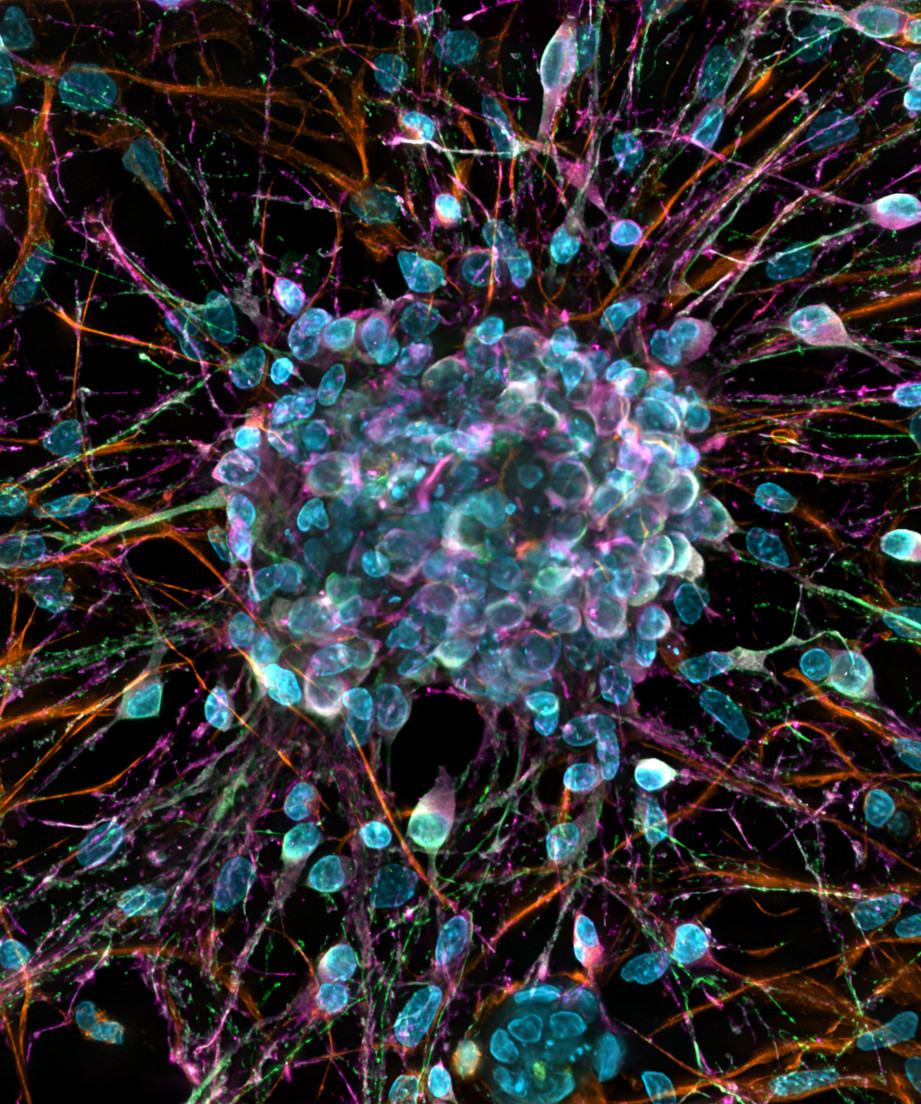
\includegraphics[width=\textwidth]{media/Rat_primary_cortical_neuron_culture_deconvolved_z-stack_overlay_(30614937102)_small.jpg}
	\end{columns}
\end{frame}

\begin{frame}{Textbook Neuron and Cell Membrane}
	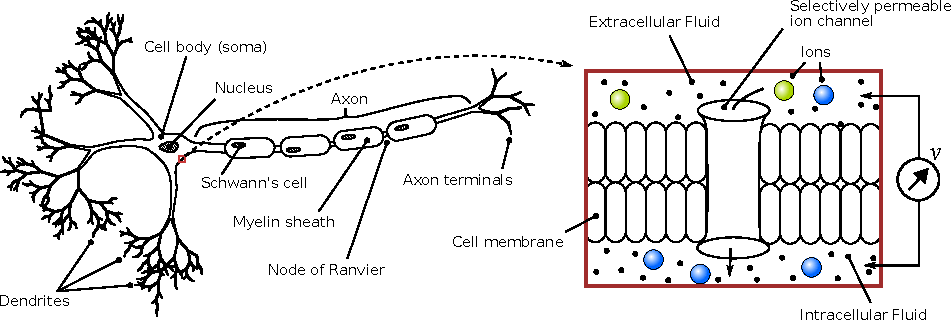
\includegraphics[width=\textwidth]{media/neuron_sketch_membrane.pdf}
\end{frame}

\begin{frame}{Injecting a Current Into a Detailed Neuron Model}
	\includegraphics<1->[width=0.5\textwidth]{media/hh_neuron_sub_threshold.pdf}%
	\includegraphics<2->[width=0.5\textwidth]{media/hh_neuron_super_threshold.pdf}

	\centering
	{\tiny\color{aluminium4} Computer simulation of an Hodgkin-Huxley type neuron with Traub kinematics (Roger D. Traub and Richard Miles, \emph{Neuronal Networks of the Hippocampus},
	Cambridge University Press, 1991)}
\end{frame}

\begin{frame}{Basic High-Level Details (Lapicque, 1907)}
	\begin{enumerate}
		\item The cell acts like a \emph{capacitor}, i.e., the voltage increases while we're injecting a current.
		\item The capacitor is \emph{leaky}. As soon as we stop injecting a current, the voltage collapses back to the resting potential $E_\mathrm{L}$.
		\item As soon as the voltage surpasses a certain value, the \emph{threshold potential} $v_\mathrm{th}$, the cell will generate a spike.
		\item Shortly after the spike has been produced, the voltage drops below the resting potential. During this period, the \emph{refractory period} of length $\tau_\mathrm{ref}$, we cannot get the neuron to spike again, even if we apply relatively large input currents $J$.
	\end{enumerate}

\end{frame}

\begin{frame}{The Leaky Integrate-and-Fire Equivalent Circuit}
	\centering
	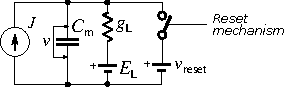
\includegraphics[width=0.7\textwidth]{media/lif_circuit.pdf}
	\begin{align}
		\begin{aligned}
			\frac{\mathrm{d}}{\mathrm{d}t} v(t) &= \frac{1}{C_\mathrm{m}} \big(g_\mathrm{L} (E_\mathrm{L} - v(t))
			+ J
			\big) \,, \quad \text{if } v(t) < v_\mathrm{th}\,.
		\end{aligned}
	\end{align}
	if $v(t) = v_\mathrm{th}$ at $t = t_\mathrm{th}$, output a spike ($\delta(t - t_\mathrm{th})$) and:
	\begin{align}
		\begin{aligned}
			v(t) &\gets v_\mathrm{reset} \,, &\text{if } t_\mathrm{th} < t \leq t_\mathrm{th} + \tau_\mathrm{ref} \,,
		\end{aligned}
		\label{eqn:super-threshold}
	\end{align}

\end{frame}

\begin{frame}{Injecting a Current Ramp into a Detailed Neuron Model}
	\centering
	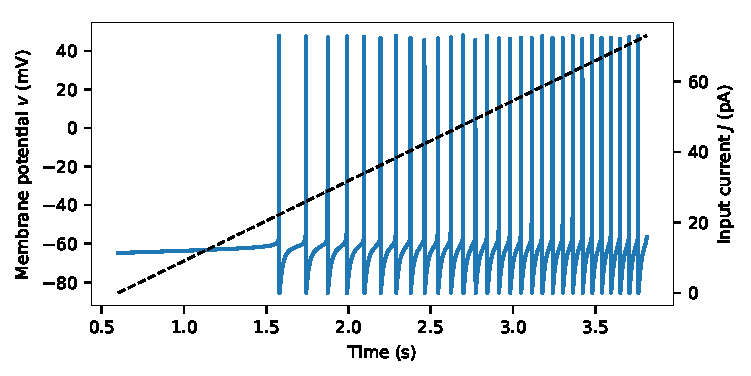
\includegraphics[width=0.9\textwidth]{media/hh_neuron_ramp.pdf}

	\begin{overlayarea}{\textwidth}{1cm}
		\centering
		{\tiny\color{aluminium4} Computer simulation of an Hodgkin-Huxley type neuron with Traub kinematics (Roger D. Traub and Richard Miles, \emph{Neuronal Networks of the Hippocampus},
			Cambridge University Press, 1991)}
	\end{overlayarea}
\end{frame}

\begin{frame}{Injecting a Current Ramp into a LIF Neuron Model}
	\centering
	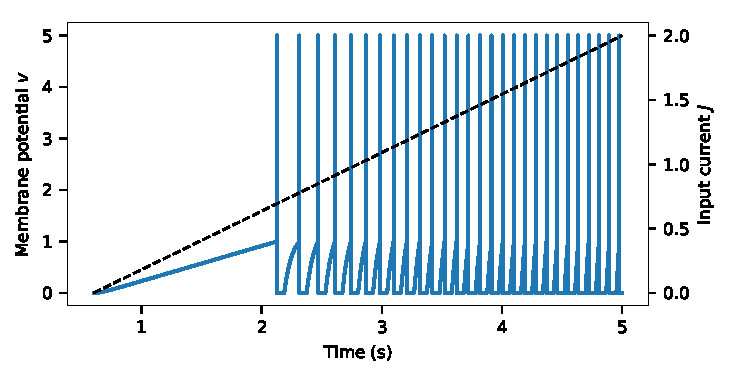
\includegraphics[width=0.9\textwidth]{media/lif_neuron_ramp.pdf} \\
	(note normalization to $v_{th}=1$, $v_{reset}=E_L=0$)

	\begin{overlayarea}{\textwidth}{1cm}
	\end{overlayarea}
\end{frame}

\begin{frame}{Limitations of the LIF Neuron Model}
	\centering
	\includegraphics<1>[width=\textwidth]{media/izhikevich_whichmod_figure1.pdf}
	\includegraphics<2>[width=\textwidth]{media/izhikevich_whichmod_figure2.pdf}
\end{frame}



\begin{frame}{LIF Rate Approximation}
	\begin{itemize}
		\item need to compute $t_\mathrm{th}$ (the time $v(t_\mathrm{th})=v_{th}$)
		\item assume: $J$ is constant and $v(0) = 0$. 
		\begin{align*}
			v(t) &= - \int_0^t \frac{1}{\tau_\mathrm{RC}} \big( v(t') - RJ \big) \,\mathrm{d}t'
			= RJ \left(1 - e^{-\frac{t}{\tau_\mathrm{RC}}} \right) \,.
		\end{align*}
		\begin{align*}
			v_\mathrm{th} = RJ \left(1 - e^{-\frac{t_\mathrm{th}}{\tau_\mathrm{RC}}} \right) 
			\Leftrightarrow 1 - \frac{v_\mathrm{th}}{RJ} = e^{-\frac{t_\mathrm{th}}{\tau_\mathrm{RC}}} \,, \\
			t_\mathrm{th} = - \tau_\mathrm{RC} \log \left( 1 - \frac{v_\mathrm{th}}{RJ} \right)
		\end{align*}
	\begin{align*}
		G[J]
		&= \begin{cases}
			\frac{1}{\tau_\mathrm{ref} - \tau_\mathrm{RC} \log \left( 1 - \frac{v_\mathrm{th}}{RJ} \right)} & \text{if } 1 - \frac{v_\mathrm{th}}{RJ} > 0 \,,\\
			0 & \mathrm{otherwise} \,.
		\end{cases}
	\end{align*}
	
	
	\end{itemize}

\end{frame}

\begin{frame}{Artifical Rate Neurons: LIF}
	\begin{columns}
		\column{0.5\textwidth}
		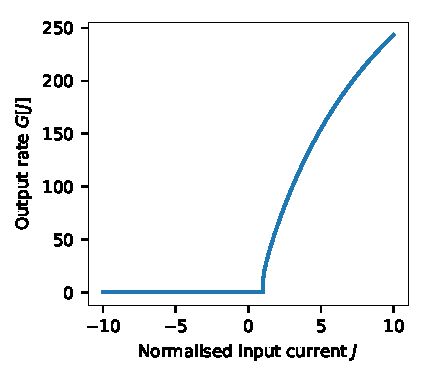
\includegraphics[width=\textwidth]{media/nonlinearity_lif.pdf}
		\column{0.5\textwidth}
		$$G[J] = \frac{1}{\tau_\mathrm{ref} - \tau_\mathrm{RC} \log\left( 1 - \frac{1}J \right)}$$\\[0.5cm]
		\textbf{Usefulness to neurobiological systems\\modellers:}
		\begin{itemize}
			\item[\OPlus] Biologically motivated
			\item[\OPlus] Captures saturation effects
			\item[\OMeh] Relatively slow to evaluate numerically (for machine-learning people)
			\item[\OMinus] Spike onset is smooth in noisy systems
		\end{itemize}
	\end{columns}	
\end{frame}



\begin{frame}{Exploring the LIF Rate Approximation}
	\centering
	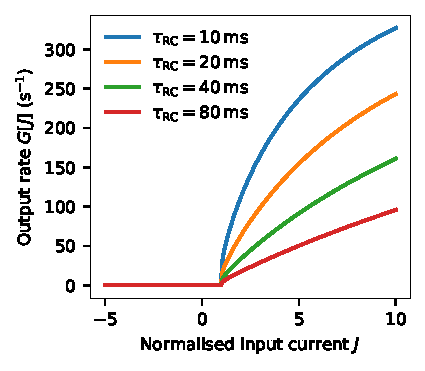
\includegraphics[width=0.5\textwidth]{media/lif_neuron_rate_tau_rc.pdf}%
	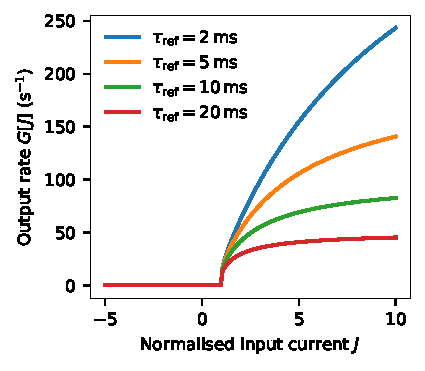
\includegraphics[width=0.5\textwidth]{media/lif_neuron_rate_tau_ref.pdf}
\end{frame}

\begin{frame}{Artifical Rate Neurons: ReLU}
	\begin{columns}
	\column{0.5\textwidth}
	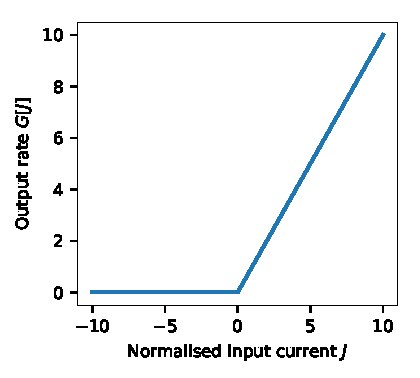
\includegraphics[width=\textwidth]{media/nonlinearity_relu.pdf}%
	\column{0.5\textwidth}
	$$G[J] = \max\{0, J\}$$\\[0.5cm]
	\textbf{Usefulness to neurobiological systems\\modellers:}
	\begin{itemize}
		\item[\OPlus] Fast to evaluate
		\item[\OMeh] Rough approximation of the LIF response curve
		\item[\OMinus] Does not capture saturation effects
		\item[\OMinus] Spike onset is smooth in noisy systems
	\end{itemize}
	\end{columns}	
\end{frame}

\begin{frame}{Artifical Rate Neurons: Smooth ReLU (Softplus)}
	\begin{columns}
	\column{0.5\textwidth}
	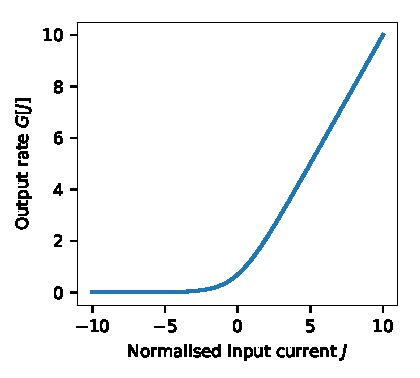
\includegraphics[width=\textwidth]{media/nonlinearity_smooth_relu.pdf}%
	\column{0.5\textwidth}
	$$G[J] = \log(1 + \exp(J))$$\\[0.5cm]
	\textbf{Usefulness to neurobiological systems\\modellers:}
	\begin{itemize}
		\item[\OPlus] Models smooth spike onset
		\item[\OMeh] Rough approximation of the LIF response curve
		\item[\OMinus] Does not capture saturation effects
	\end{itemize}
	\end{columns}	
\end{frame}

\begin{frame}{Artifical Rate Neurons: Logistic Function}
	\begin{columns}
	\column{0.5\textwidth}
	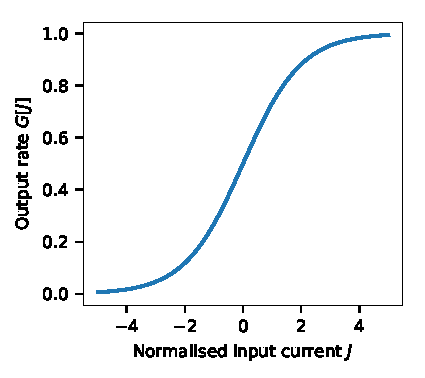
\includegraphics[width=\textwidth]{media/nonlinearity_logistic.pdf}%
	\column{0.5\textwidth}
	$$G[J] = \frac{1}{1 + e^{-J}}$$\\[0.5cm]
	\textbf{Usefulness to neurobiological systems\\modellers:}
	\begin{itemize}
		\item[\OMeh] Models smooth spike onset and saturation (?)
	\end{itemize}
	\end{columns}	
\end{frame}

\begin{frame}{Artifical Rate Neurons: Hyperbolic Tangent}
	\begin{columns}
	\column{0.5\textwidth}
	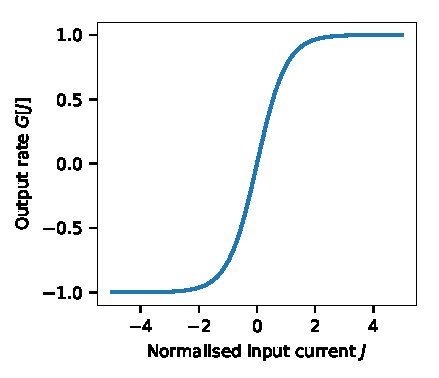
\includegraphics[width=\textwidth]{media/nonlinearity_tanh.pdf}%
	\column{0.5\textwidth}
	$$G[J] = \tanh(J) = \frac{e^J - e^{-J}}{e^J + e^{-J}}$$\\[0.5cm]
	\textbf{Usefulness to neurobiological systems\\modellers:}
	\begin{itemize}
		\item[\OMeh] Models smooth spike onset and saturation (?)
		\item[\OMinus] Negative rates
	\end{itemize}
	\end{columns}	
\end{frame}

\backupbegin

\begin{frame}[noframenumbering]{Image sources}
	\small
	\textbf{Title slide}\\Image of rat primary cortical neurons in culture.\\Author: ZEISS Microscopy, \url{http://www.zeiss.com/celldiscoverer}.\\From \href{https://commons.wikimedia.org/wiki/File:Rat_primary_cortical_neuron_culture,_deconvolved_z-stack_overlay_(30614937102).jpg}{Wikimedia}.
\end{frame}

\backupend

\end{document}
